\clearpage
\setcounter{page}{1}
\maketitlesupplementary

\appendix
\section{VLA 결정의 확정 규칙 (M4)}
\label{sec:supp_m4}
\begin{figure*}[t]
\centering
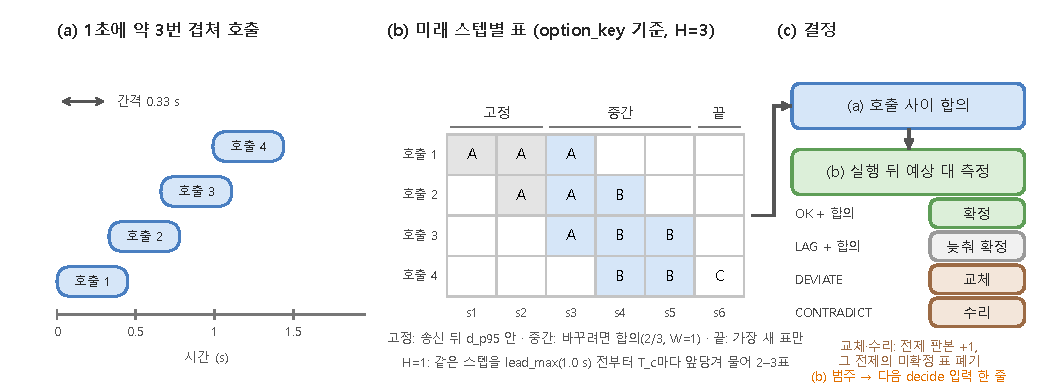
\includegraphics[width=\linewidth]{figures/m4_commit.pdf}
\caption{\textbf{M4 확정 규칙.} (a) Jev를 약 0.33\,s 간격으로 겹쳐 부른다(지연은 E0에서 실측). (b) 답을 미래 스텝별 표로 모으고, RTC의 구간을 이산판으로 옮겨 고정(Jev p95 지연 길이), 중간(바꾸려면 합의 필요), 끝(최신 표 가확정)으로 나눈다. 표의 보기는 \texttt{option\_key}로 센다. (c) 호출 사이 합의(a)와 실행 뒤 코드 예상 상태 대 측정 상태 비교(b)가 모두 맞으면 확정하고, (b)가 어긋나면 전제 판본을 올려 그 전제에 기댄 표를 무효화한 뒤 교체·수리를 고른다. 표의 A--D는 설명용 예시다.}
\label{fig:m4}
\end{figure*}

결정 호출은 로봇 동작보다 느리므로 약 0.33\,s 간격으로 겹쳐 부르고, 겹쳐 받은 답을 미래 스텝별 ``표''로 원장에 쌓는다(\cref{fig:m4}). 이미 시작한 스텝은 바꾸지 않고(고정 구간), 중간 구간은 합의가 있어야 바꾸며, 끝 구간은 가장 새 표를 가확정한다. 구간 설계는 RTC~\cite{black2025rtc}의 구간을 이산 결정으로 옮긴 것이다.

\paragraph{(a) 호출 사이 합의.} 스텝 $s$의 살아 있는 표가 $n_s$개이고 현 선택과 일치하는 표가 $m_s$개일 때, 최근 두 표가 같거나($\text{LA-2}$) $n_s\ge3$이면서 $3m_s\ge2n_s$이면 확정 후보가 된다. 다른 보기를 고른 도전 표는 첫 도전 표 뒤에 같은 도전 표가 하나 더 와야 현 선택을 바꾼다. 되돌릴 수 없는 보기는 하나 더 요구한다. 전제 판본이 오래된 표와 나이 1.5\,s를 넘은 표는 버린다.

\paragraph{(b) 실행 뒤 확인.} 스텝을 실행한 뒤, 확정 청크의 기준 궤적 대비 측정 손끝의 잔차와, 선택 보기의 예상 결과 술어가 스텝 끝에 성립하는지를 본다. 결과는 OK, LAG(늦지만 방향이 맞음), DEVIATE(이탈), CONTRADICT(예상 술어와 모순)다. 로봇 쪽 술어(그리퍼 열림, 쥠, 쥔 채 들림)는 그리퍼 폭·전류로 코드가 판정하고(T1), 세계 쪽 술어는 같은 백본의 확인 헤드 V1h가 판정한다. 범주는 다음 결정 요청의 마지막 줄(\texttt{last\_step})로 결정 모델에 되먹인다.

\paragraph{유지·교체·수리.} (a)와 (b)의 조합마다 할 일을 정한다(\cref{tab:m4rule}). 어느 경우에도 로봇을 멈추지 않으며, 정지와 복구는 critic의 실패 판정을 거쳐야만 일어난다. 같은 모델은 같은 오답을 반복할 수 있어 (a)만으로는 부족하다. 이미 실행한 동작의 측정인 (b)가 원장의 전제를 무효화한다는 점이 같은 시각 샘플 합의~\cite{a3commit2026}와 다르다. 결합 사전 실행에서 드러난 멈춤 고리(고유 감각 모순 $\rightarrow$ 보류 $\rightarrow$ 결정 비움 $\rightarrow$ 청크 정지)는 이 규칙의 보류 경로에서 생겼고, 보류 탈출·그리퍼 열림 이력·쥐는 동안 마지막 청크 유지로 고쳤다(폐루프 확인 \tentative{예정}).

\begin{table}[t]
\centering
\scriptsize
\setlength{\tabcolsep}{3pt}
\begin{tabular}{@{}p{0.17\linewidth}p{0.22\linewidth}p{0.19\linewidth}p{0.26\linewidth}@{}}
\toprule
(b) \textbackslash{} (a) & 합의 & 경합 & 불일치 급증 \\
\midrule
OK & 확정 & 유지, 유예 창 진행 & 확정 중단, 조기 호출 \\
LAG & 확정, 시각만 뒤로 & 유지 & 조기 호출 \\
DEVIATE & 판본$+1$, 미확정 표 폐기, 교체 & 교체 & 교체, 조기 호출 \\
CONTRA\-DICT & \multicolumn{3}{p{0.67\linewidth}@{}}{판본$+1$, 미확정 표 폐기, 직전 확정 행동 유지 + 감속, critic에 신호} \\
\bottomrule
\end{tabular}
\caption{\textbf{M4 결정 표.} M4는 신호만 내고 실패는 critic이 판정한다.}
\label{tab:m4rule}
\end{table}

\paragraph{절제 계획 (E-M4).} 같은 초당 호출 수에서 섭동 4종 $\times$ 30회 이상 $\times$ 3시드로, 기다림(C0), 요청 하나 + 직전 행동 유지(C1), 가장 새 답(C2~\cite{slowbrain2026}), 확률 융합(C2$'$), 같은 시각 샘플 합의(C5-A3), (a)만(C3), (b)만(C4), 둘 다(C5), C5에서 (b) 되먹임 뺌(C5$'$)을 비교한다. 주 지표는 섭동 성공률, 잘못 확정 비율, 섭동 반응 시간이며, 결과 칸은 예정이다. 판정 초안은 C5가 C2와 C2$'$보다 \tentative{+10\%p}(하한 $>0$) 높거나, 비슷하면서 잘못 확정이 상대 \tentative{30\%} 이상 낮을 때 확정 규칙의 기여를 주장하는 것이다.

\section{재현성, 사전 등록, 감사}
\label{sec:supp_repro}
\paragraph{시뮬 재현성.} CPU PhysX는 환경 리셋을 넘어 장면 내부 상태를 이어 가, 같은 시드가 직전 실행 이력에 따라 몇 개의 이산 궤적 가운데 하나로 재생되었다(물체 최대 편차 \tentative{4--39\,mm}). 매 에피소드 시작에서 물리 장면을 다시 만들자, 서로 다른 이력 뒤의 실행이 새 프로세스의 실행과 매 틱 비트 단위로 같아졌다(\tentative{24/24}, 에피소드당 \tentative{약 0.28\,s}). 렌더 픽셀은 물리 상태가 같아도 비트 단위로 같지 않았다. 스냅샷에서 분기한 라벨은 복원이 비트 단위로 같을 때만 믿는다.

\paragraph{사전 등록과 자체 검사.} 모든 실험은 실행 전에 바꾸는 설계 결정, 표본으로 그 결정을 가를 수 있는지, 판정 문턱, 판정 스크립트를 커밋한다. 결과를 본 뒤의 선택은 새 등록과 새 표본으로만 확인한다. 결정 확신도가 그 예다. 판정 밖 기준선에서 좋았지만(\tentative{0.804}), 새 표본 등록에서 실데이터 문턱을 넘지 못해 채택하지 않았다. 과금되는 호출은 사용자의 명시적 허락 뒤에만 한다.

\paragraph{적합성 감사.} 독립 검증 에이전트가 등록 문서에서 대조표를 새로 만들어 평가 코드가 숫자와 조건 문장을 그대로 구현하는지 확인한다. 두 번 연속 결함 없이 끝나야 통과이며, \tentative{37}회차 가운데 36·37회차가 연속으로 통과해 파이프라인 기준점을 고정했다. 감사는 실행 확인만으로는 보이지 않던 불일치를 여러 건 찾았다. 합의 비율 0.67을 소수로 비교해 ``세 표 중 두 표''가 확정되지 않던 것, 기준 조건의 정의가 등록과 다르던 것 등이다.

\section{입력 형식 시험과 채택하지 않은 보강}
\label{sec:supp_tests}
아래는 입력 형식과 학습 보강을 고르기 위한 소규모 시험이다. 공개 실물 데이터에서 돈 시험은 파이프라인 시험이며, 수치는 형식 선택에만 쓰고 결과로 쓰지 않는다(\cref{tab:supptests}).

\begin{table*}[t]
\centering
\scriptsize
\setlength{\tabcolsep}{3pt}
\begin{tabular}{@{}p{0.17\linewidth}p{0.30\linewidth}p{0.33\linewidth}p{0.14\linewidth}@{}}
\toprule
시험 & 조건 & 값 (파이프라인 시험 또는 초기값) & 결정 \\
\midrule
움직임 줄 & 공개 실물, 2$\times$2 뒤 두 시드 확인, 검증 1,799 & \tentative{+0.032} [\tentative{+0.022, +0.043}], 전환 층 \tentative{+0.030} & 채택 \\
2프레임 비디오 & 같은 2$\times$2 & \tentative{+0.013}, 전처리 포함 p95 \tentative{+20\%} & 불채택 \\
VLA 카메라 3대 & 공개 실물, 두 시드 & \tentative{+0.0014}, p95 \tentative{+11.7\%} & 불채택 \\
3D 미래 손끝 궤적 보조 & 공개 실물, 두 시드 & \tentative{+0.0031} [\tentative{$-$0.0022, +0.0085}] & 불채택 \\
2D 궤적 보조(포인팅 라벨) & 공개 실물, 거르개 v2 라벨 & \tentative{+0.0047} [\tentative{$-$0.0006, +0.0103}] & 불채택 \\
전문가 층별 KV 조건 & 공개 실물, 두 시드 & 청크 오차 \tentative{$-$2.19\%}(문턱 5\%) & 불채택 \\
명령을 VLA 입력에 & 시뮬, 문장·화살표 명령 & 반사실 준수 \tentative{0.177}, \tentative{0.0008}(문턱 0.6) & 불채택(코드 편향만) \\
결정 드롭아웃 + CFG, 되짚기 라벨 & 시뮬, 두 시드 & 최고 \tentative{0.598}, 청크·그리퍼 비열등 실패 & 불채택 \\
백본 특징 새로움 & 시뮬 평가 7,308 & 큰 오류 AUROC \tentative{0.570} & 불채택 \\
결정 확신도(새 표본) & 시뮬 새 표본, 실데이터 1,799 & \tentative{0.806}, \tentative{0.748} & 기록만 \\
영점 선택기 & 학습 안 한 4B, DEV 스냅샷 & \tentative{0.483} $<$ 최빈 \tentative{0.669} & 기준선 행만 \\
명시적 인식 & SAM 3.1 + 렌더 깊이 & 3D 중심 오차 중앙 \tentative{35\,mm} & 런타임에서 뺌 \\
\bottomrule
\end{tabular}
\caption{\textbf{입력 형식 시험과 채택하지 않은 보강.} 모두 사전 등록 판정이다. 공개 실물 데이터의 값은 휴리스틱 라벨 위의 파이프라인 시험이라 형식 선택에만 쓴다. MolmoAct식 조각이 효과가 없었던 데는 원 논문의 성립 조건을 갖추기 전에 옮긴 탓이 섞여 있다.}
\label{tab:supptests}
\end{table*}

\section{비용 모형}
\label{sec:supp_cost}
직렬 흐름의 호출 수는 판 길이 $T$와 지연 $L$로 $T/L$이고, 비용은 호출 수 $\times$ 호출당 비용이다. 탐침에서 흐름 호출은 \tentative{약 50--58원}이었으므로 로봇 1분당 \tentative{약 350--500원}이다. 동기 단독 팔은 성공 1편에 \tentative{약 590원}이 들었다. 학생 상위 모델은 로컬 GPU에서 돌아 API 비용이 0이며, 이것이 가설 H-L의 동기 가운데 하나다.
